\section{Appendix}
\subsection{Target accuracy : code}
\label{appendix:targetaccuracy}
\begin{lstlisting}[language=Python]
from sklearn.ensemble import RandomForestClassifier
pipe_test = Pipeline([('scaler', StandardScaler()), ('rf', RandomForestClassifier())])
parameters_test = {'rf__n_estimators':[100,150],
                   'rf__criterion': ['gini','entropy']} 
scoring_test = {'accuracy': make_scorer(accuracy_score)}
clf_test = GridSearchCV(pipe_test, parameters_test, cv=3,scoring = scoring_test, refit='accuracy')
clf_test.fit(X_train, y_train)
print('Returned hyperparameter: {}'.format(clf_test.best_params_))
print('Best classification accuracy in train is: {}'.format(clf_test.best_score_))
print('Classification accuracy on test is: {}'.format(clf_test.score(X_test, y_test)))
\end{lstlisting}

\subsection{Visualizing Errors : code chunk}
\label{appendix:visualizing}
\begin{lstlisting}[language=Python]
axes = plt.subplots(2, 4)[1]  # creates a grid of 10 plots

# More details about zip() function here https://docs.python.org/3.3/library/functions.html#zip
y_pred = clf4.predict(X_test)
j = 0 # Index which iterates over plots
for true_label, pred_label, image in list(zip(y_test, y_pred, X_test)):
    if j == 4: # We only want to look at 4 first mistakes
        break
    if true_label != pred_label:
        # Plotting predicted probabilities
        axes[1, j].bar(np.arange(10), clf4.predict_proba(image.reshape(1, -1))[0]) 
        axes[1, j].set_xticks(np.arange(10))
        axes[1, j].set_yticks([])
        
        # Plotting the image
        axes[0, j].imshow(image.reshape((28, 28)), cmap=plt.cm.gray_r, interpolation='nearest')
        axes[0, j].set_xticks([])
        axes[0, j].set_yticks([])
        axes[0, j].set_title('Predicted {}'.format(pred_label)+'/True {}'.format(true_label),fontsize=8)
        j += 1
\end{lstlisting}
	
\begin{figure*}[h]
	\centering 
	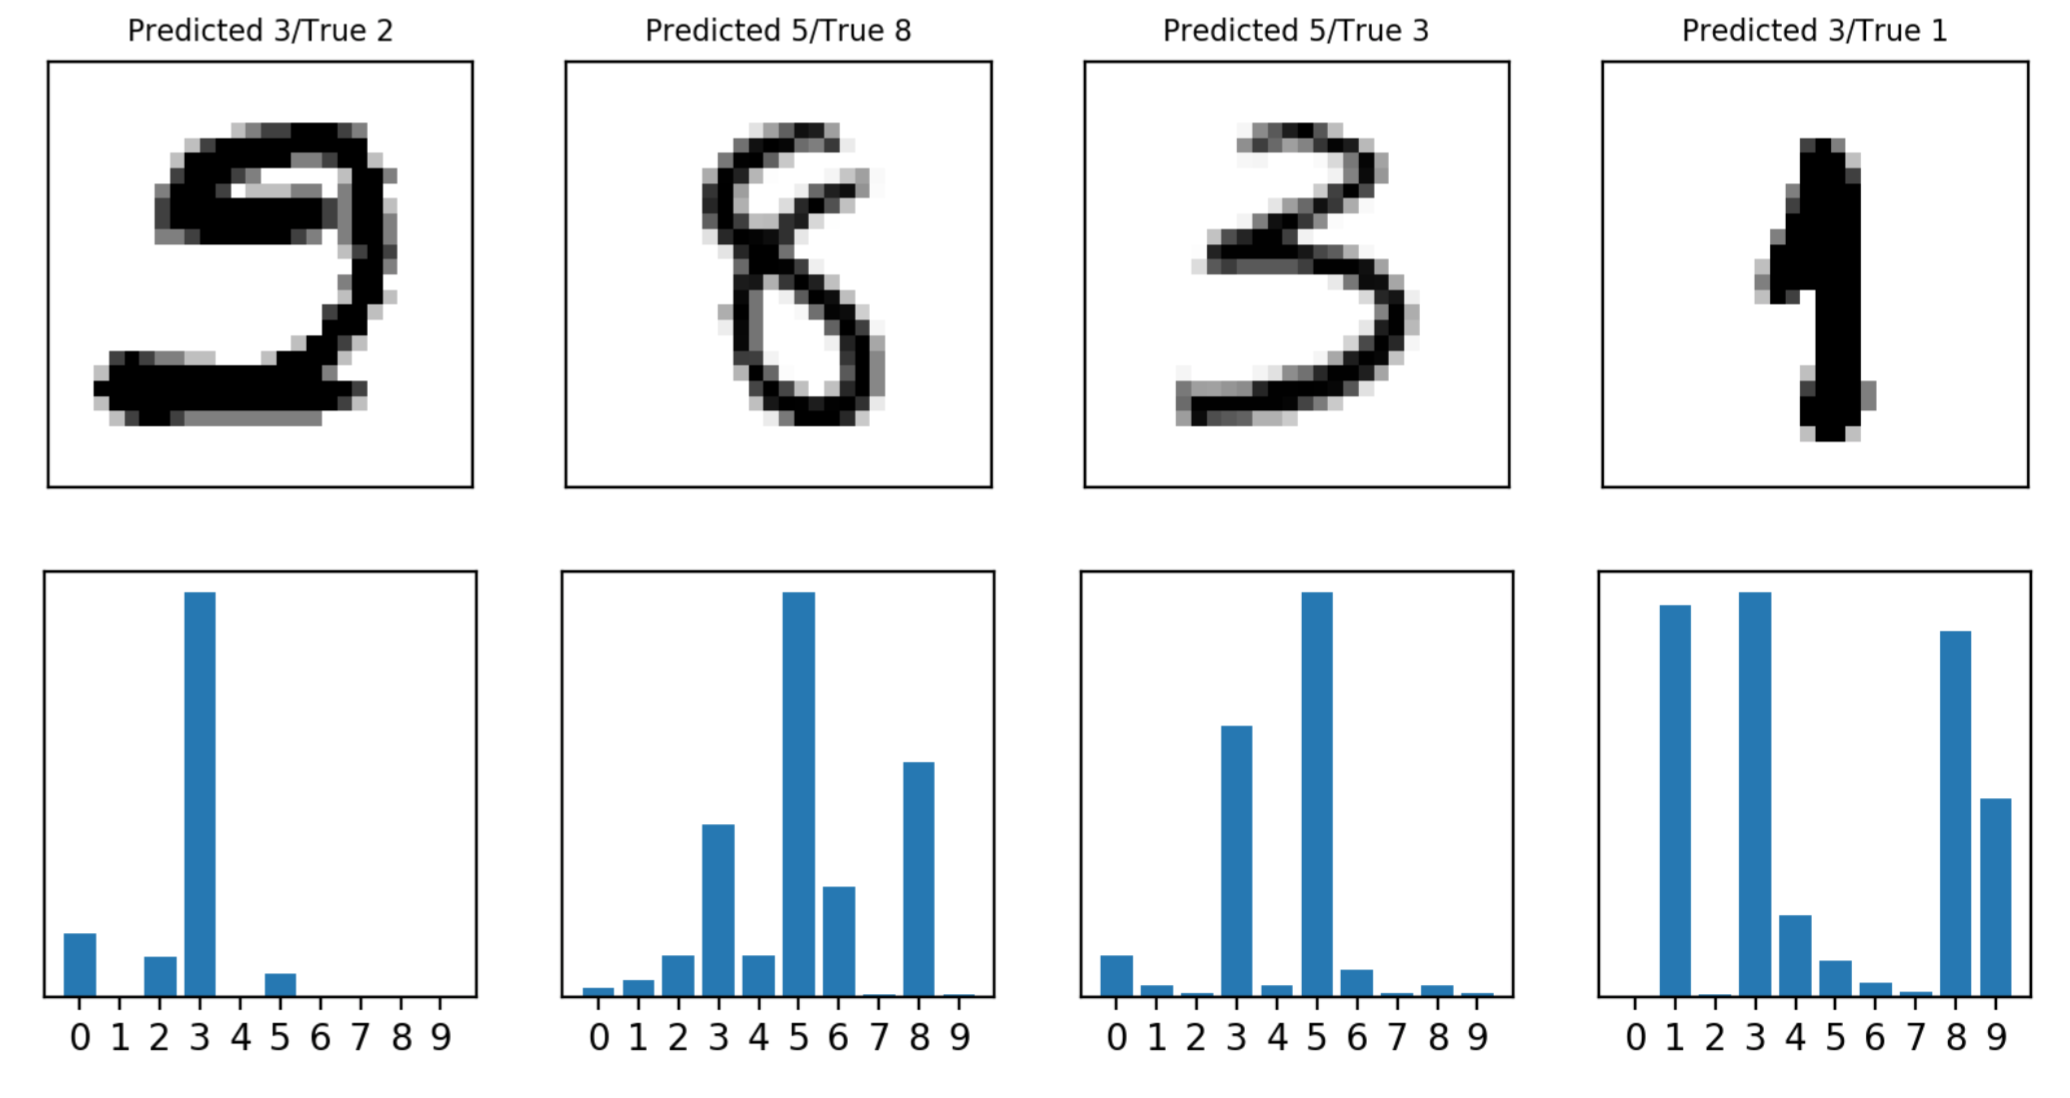
\includegraphics[scale=0.35]{Pics/probas}
	\caption{Probabilities of each outcome for the logistic regression}
	\label{fig:probas}
\end{figure*}



\newpage

\subsection{Changing the loss function : confusion matrix / heatmap}
\label{appendix:changingloss}
\begin{figure*}[h]
	\centering 
	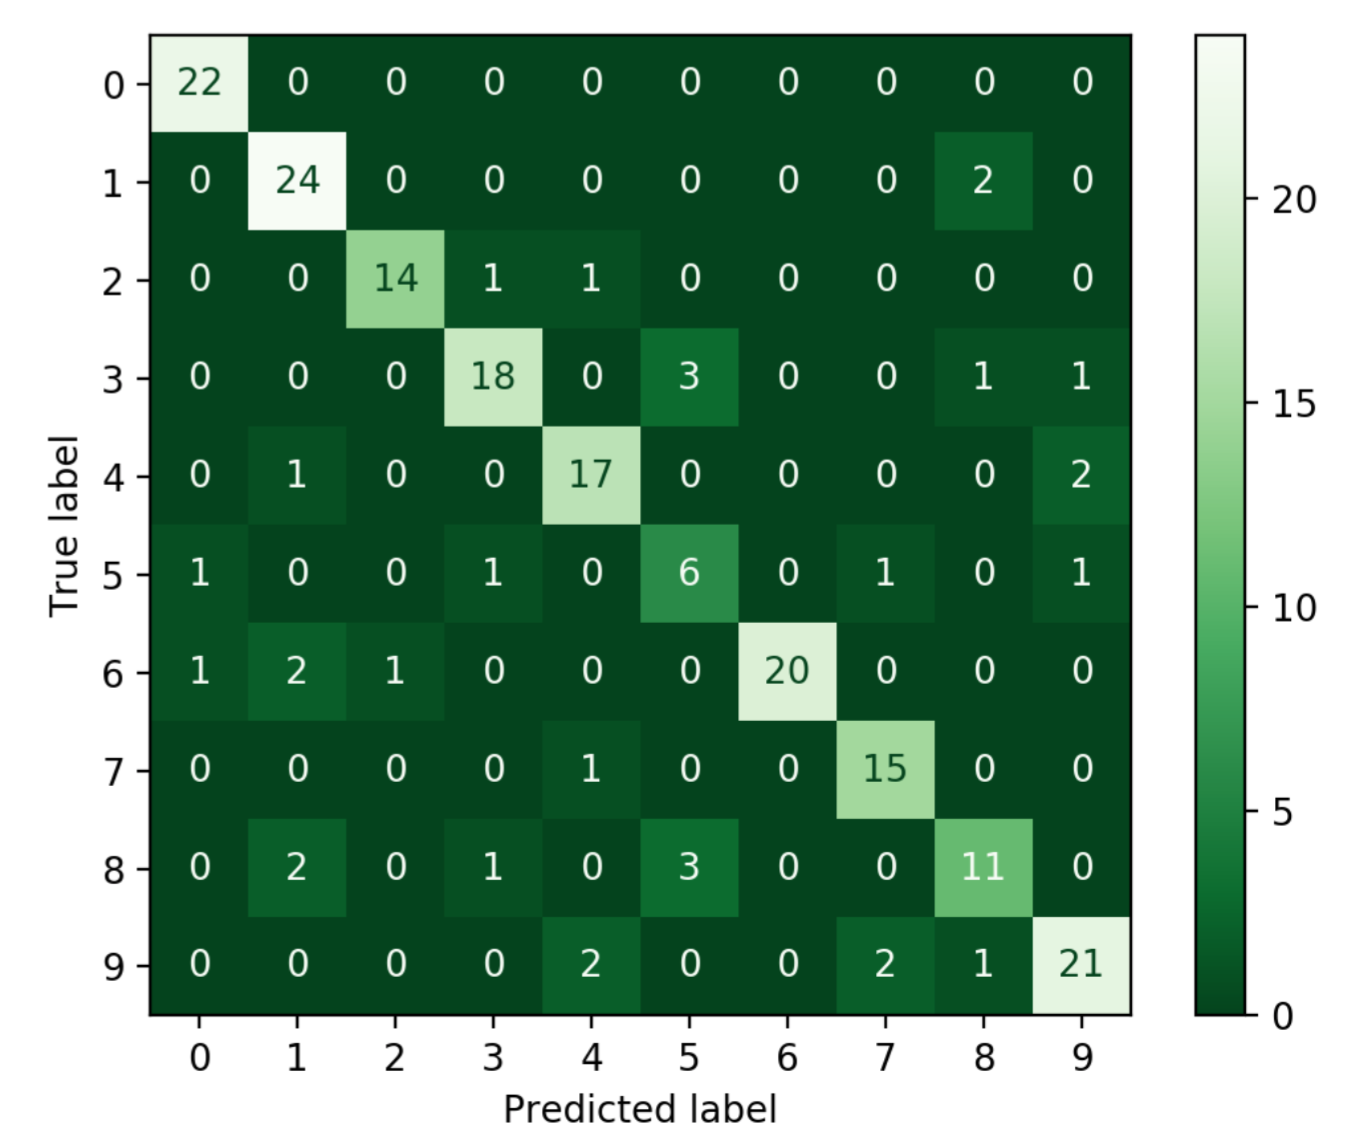
\includegraphics[scale=0.4]{Pics/confusion_matrixr}
	\caption{Confusion matrix for the SVM classifier}
	\label{fig:confusion}
\end{figure*}


\subsection{Part 2 : code}
\label{appendix:code_part2}
\begin{lstlisting}[language=Python]
def custom_MNISTscorer(y_true, y_predict):
    #Classe 1 : les chiffres 0:4, Classe 0 : les chiffres 5:9
    y_predict_class = (np.array(y_predict).astype(int)<5).astype(int)
    y_true_class = (np.array(y_true).astype(int)<5).astype(int)
    
    #Compute accuracy for class 0 - 1 and labels 0:9
    Class_weightedaccuracy = sklearn.metrics.balanced_accuracy_score(y_true_class, y_predict_class)
    Label_weightedaccuracy = sklearn.metrics.balanced_accuracy_score(y_true, y_predict)
    return Label_weightedaccuracy * Class_weightedaccuracy
\end{lstlisting}

\subsection{Part 2 : final confusion matrix}
\begin{figure*}[h]
	\centering 
	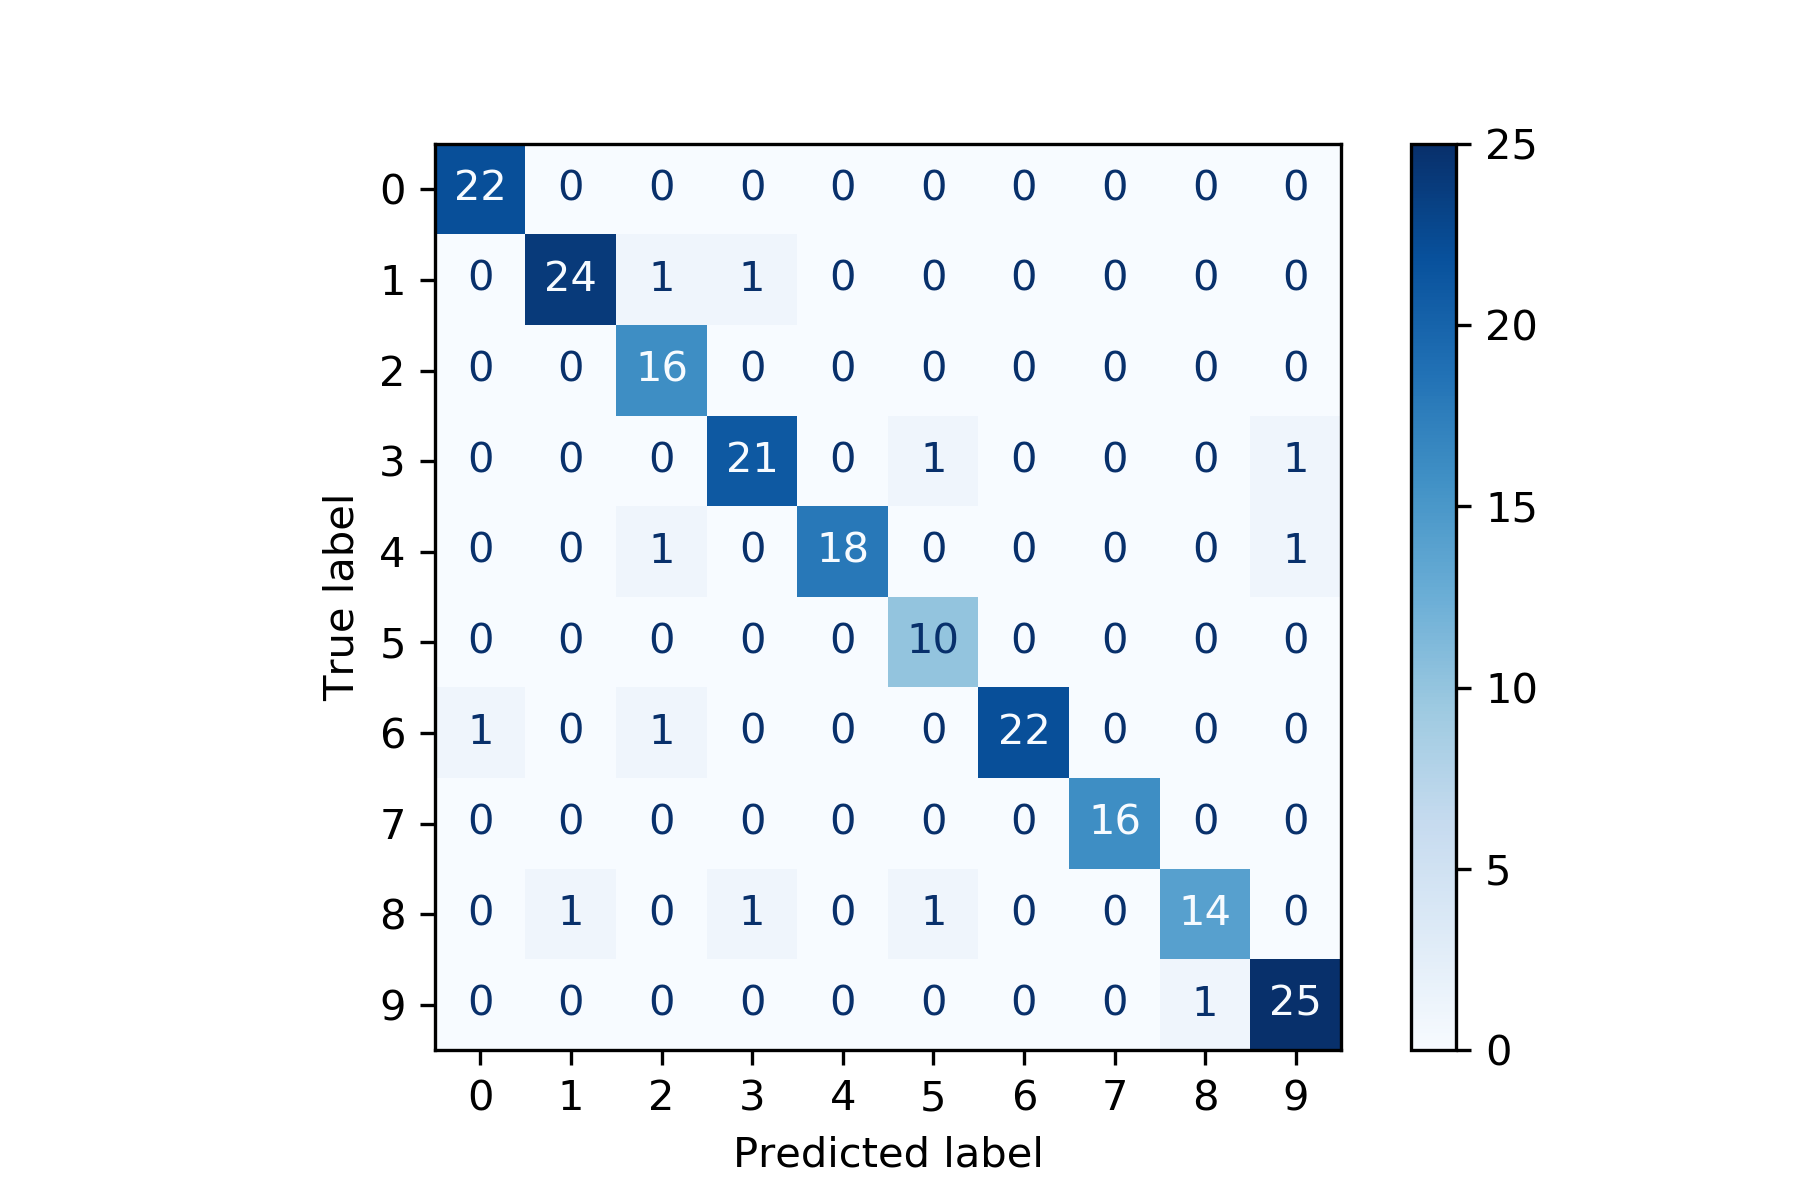
\includegraphics[scale=0.7]{Pics/part2confusion_mat}
	\caption{Confusion matrix part 2}
	\label{fig:confusion}
\end{figure*} 

\begin{figure*}[h]
	\centering 
	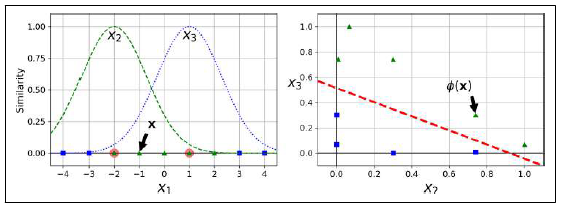
\includegraphics[scale=0.7]{Pics/RBF}
	\caption{Similarity features using the Gaussian RBF}
\end{figure*} 
